\documentclass[12pt, answers,fleqn]{exam}
\usepackage{pifont}
\usepackage{dingbat}
\usepackage{amsmath,amssymb}
\usepackage{epsfig}
\usepackage[super]{nth}
\usepackage[colorlinks=true,linkcolor=black,anchorcolor=black,citecolor=black,filecolor=black,menucolor=black,runcolor=black,urlcolor=black]{hyperref}
\usepackage[letterpaper, margin=0.75in]{geometry}
\addpoints
\boxedpoints
\pointsinmargin
\pointname{pts}

\usepackage[activate={true,nocompatibility},final,tracking=true,kerning=true,factor=1100,stretch=10,shrink=10]{microtype}
\usepackage[american]{babel}
%\usepackage[T1]{fontenc}
\usepackage{fourier}
\usepackage{isomath}
\usepackage{upgreek,amsmath}
\usepackage{amssymb}
\usepackage{graphicx}

\newcommand{\dotprod}{\, {\scriptzcriptztyle
    \stackrel{\bullet}{{}}}\,}

\newcommand{\reals}{\mathbf{R}}
\newcommand{\lub}{\mathrm{lub}} 
\newcommand{\glb}{\mathrm{glb}} 
\newcommand{\complex}{\mathbf{C}}
\newcommand{\dom}{\mbox{dom}}
\newcommand{\range}{\mbox{range}}
\newcommand{\cover}{{\mathcal C}}
\newcommand{\integers}{\mathbf{Z}}
\newcommand{\vi}{\, \mathbf{i}}
\newcommand{\vj}{\, \mathbf{j}}
\newcommand{\vk}{\, \mathbf{k}}
\newcommand{\bi}{\, \mathbf{i}}
\newcommand{\bj}{\, \mathbf{j}}
\newcommand{\bk}{\, \mathbf{k}}
\DeclareMathOperator{\Arg}{\mathrm{Arg}}
\DeclareMathOperator{\Ln}{\mathrm{Ln}}
\newcommand{\imag}{\, \mathrm{i}}

\usepackage{graphicx}
\usepackage{color}
\shadedsolutions
\definecolor{SolutionColor}{rgb}{0.8,0.9,1}
\newcommand\AM{\textsc{am}}
\newcommand\PM{\textsc{pm}}
     
\newcommand{\quiz}{Review Exam I}
\newcommand{\term}{Fall}
\newcommand{\due}{Wednesday 31 August at 13:15 \PM}
\newcommand{\class}{MATH 115}
\begin{document}
\large


\vspace{0.1in}
\noindent{\textbf{Review for Exam I}}

\begin{questions} 

    \large


\question Larry claims that it is true that
$\displaystyle
    \lim_{x \to \sqrt{7}} \lfloor x \rfloor = \lfloor \sqrt{7} \rfloor,
$
but Larry can't remember the justification for this calculation. Explain to 
Larry what function property justifies this calculation. Write your answer in
sentence form.
\begin{solution} Larry used \emph{direct substitution} to evaluate this limit. Direct
    substitution is justified provided the function is \emph{continuous} at the limit 
    point.  Here the limit point is $\sqrt{7}$. The floor function is continuous 
    at $\sqrt{7}$, so direct substitution is justified.    
\end{solution}

\question Find the value of \(\displaystyle \lim_{x \to \uppi} 
\left(5 \lfloor x \rfloor -  \lfloor 5 x \rfloor  \right) \).
\begin{solution} The floor function is continuous at $\uppi$ and at $5 \uppi$. Thus
    \[
    \lim_{x \to \uppi} 
\left(5 \lfloor x \rfloor -  \lfloor 5 x \rfloor  \right) 
 = 5 \lfloor \uppi \rfloor -  \lfloor 5 \uppi \rfloor
 = 0.
    \]
Although you might guess that $5 \lfloor x \rfloor -  \lfloor 5 x \rfloor = $
for all real $x$, that's rubbish. For example, 
$5 \lfloor 3/2 \rfloor -  \lfloor 5 \times 3/2 \rfloor = -2$. Actually,
the graph of $y = 5 \lfloor x \rfloor -  \lfloor 5 x \rfloor$ is a curious
thing--you should look at it sometime.
\end{solution}

\question Define a function $A(x) = x^2 |x|$. Use the definition of
the derivative as a limit of a Newton quotient to find the value of $A^\prime(0)$.
\begin{solution}   
    \[
        \lim_{x \to 0} \frac{A(x) - A(0)}{x-0} =
    \lim_{x \to 0} \frac{x^2 |x| - 0}{x-0} = \lim_{x \to 0} x |x| = 0.
    \]
The last step is justified in part by the fact that the absolute value
function is continuous everywhere. That makes direct substitution OK.
\end{solution}
\question Find the value of \(\displaystyle \lim_{x \to 2^{(-)}} 
 \lfloor x \rfloor \).
\begin{solution}
For $x$ near, but to the left of two, \(\lfloor x \rfloor \) simplifies
to one. Thus
\[
    \lim_{x \to 2^{(-)}}  \lfloor x \rfloor = \lim_{x \to 2^{(-)}} 1 = 1.
\]
\end{solution}
\question The \emph{domain} of the natural exponential function is \underline{\phantom{xxxxxxxxx}}.
\begin{solution}
    The \emph{domain} of the natural exponential function is $\reals$.
\end{solution}
\question The \emph{range} of the natural exponential function is  \underline{\phantom{xxxxxxxxx}}.
\begin{solution}
    The \emph{range} of the natural exponential function is $(0,\infty)$.
\end{solution}
    
\question The \emph{domain} of the natural logarithm function is \underline{\phantom{xxxxxxxxx}}.
\begin{solution}
    The \emph{domain} of the natural logarithm function is  \((0,\infty)\).
\end{solution}
\question The \emph{range} of the natural logarithm function is    \underline{\phantom{xxxxxxxxx}}.
\begin{solution}
    The \emph{range} of the natural logarithm function is $(-\infty, \infty)$.
\end{solution}
\question Find an equation of the tangent line (TL) to the curve  $y = x (x-4)$. 
The point of tangency is $(x= 5, y=5)$.
\begin{solution}
    We need a point on the line and its slope.  The point is given--it is \mbox{$(x= 5, y=5)$}.
    To find the slope of the TL, we need to evaluate 
    \[
    \left. \frac{\mathrm{d}y}{\mathrm{d}x} \right \vert_{x=5} = 
    \left. 2x - 4\right \vert_{x=5}  = 6. 
    \]
    So an equation for the TL is $y-5 = 6(x-5).$  Since the problem
    asked for ``an equation of the tangent line,'' you are
    free to present your answer in either point-slope form,
    intercept form, or general form.  Isn't freedom of
    expression \emph{wonderful?}
    
\end{solution}
\question Find an equation of the tangent line (TL) to the curve $y = \mathrm{e}^x$. 
The point of tangency is $(x= 0, y=1)$.
\begin{solution}
    We need a point on the line and its slope.  The point is given--it is \mbox{$(x= 0, y=1)$}.
    To find the slope of the TL, we need to evaluate $\displaystyle
    \left. \frac{\mathrm{d}y}{\mathrm{d}x} \right \vert_{x=0} = 
    \left. \mathrm{e}^x \right \vert_{x=0}  = 1.$ So an equation for the 
    TL is $y-1 = x$
    
\end{solution}

\question Find the \emph{natural domain} of the function whose formula is $W(x) = \frac{5}{x} - \frac{x}{5}$.
\begin{solution}
    There is only one denominator that can vanish; thus
    \(
     \dom{W} = \{x | x \neq 0 \}.
    \)
    
\end{solution}

\question Find the \emph{natural domain} of the function whose formula is 
$Q(x) = \frac{5}{1 - \frac{1}{x}} $.
\begin{solution}
    There are two denominators--we need both of them to be nonzero. Thus
    \[
         \left \{x |  \,\,  1 - \frac{1}{x} \neq 0 \mbox{ and } x \neq 0 \right \}
       =  \left \{x |   x \neq 1 \mbox{ and } x \neq 0 \right \}.
    \]

    Remember that \(\left \{x |  \,\,  1 - \frac{1}{x} \neq 0 \mbox{ and } x \neq 0  \right \} \)
    is in \emph{implicit form}, so it is \textbf{not} simplified and it
    is \textbf{unworthy} of earning full credit.

    \quad Also, the problem statement does not mandate the way to express 
    the answer, so you have the \textbf{freedom} to present your
    answer in either set builder notation, interval notation, or pictorially.
    \textbf{It's all good!} In interval notation, the solution is \((-\infty,0) \cup (0,1) \cup (1,\infty) \).


    \textbf{Careful:} If you ``simplify'' $\frac{5}{1 - \frac{1}{x}}$ To
    $\frac{5x}{x - 1}$, you will miss the fact that zero is 
    not in the natural domain.  
\end{solution}
\question Find each derivative

\begin{parts}

    \part \(\frac{\mathrm{d}}{\mathrm{d} x} \left[ \sqrt{107} \right] \)
    \begin{solution}%[2.5in]
    Ha! Don't get caught using the power rule! This is the derivative of
    a constant, so \(\frac{\mathrm{d}}{\mathrm{d} x} \left[ \sqrt{107} \right] = 0.\)

    \end{solution}
    \part \(\frac{\mathrm{d}}{\mathrm{d} x} \left[ 2 x^2 + 31 x + 107 \right] \)
    \begin{solution}%[2.5in]
    We have
    \[
        \frac{\mathrm{d}}{\mathrm{d} x} \left[ 2 x^2 + 31 x + 107 \right]  = 4 x + 31. 
    \]

    \end{solution}

    \part \(\frac{\mathrm{d}}{\mathrm{d} x} \left[ \sqrt{2} x - \sqrt{2 x} \right] \)
    \begin{solution}%[2.5in]
        We have 
        \[
            \frac{\mathrm{d}}{\mathrm{d} x} \left[ \sqrt{2} x - \sqrt{2 x} \right]
             = \frac{\mathrm{d}}{\mathrm{d} x} \left[ \sqrt{2} x - \sqrt{2} \sqrt{x} \right] 
             = \sqrt{2} - \frac{\sqrt{2}}{2 \sqrt{x}}.
        \]
    
    \end{solution}

    \part \(\frac{\mathrm{d}}{\mathrm{d} x} \left[ (x-5)(x-7) \right] \)
    \begin{solution}%[2.5in]
    Via the product rule
    \[
        \frac{\mathrm{d}}{\mathrm{d} x} \left[ (x-5)(x-7) \right]
        =  (x-5)^\prime (x-7) + (x-5)(x-7)^\prime = (x-7)+(x-5)= 2 x - 12.
    \]
    \end{solution}

    \part \(\frac{\mathrm{d}}{\mathrm{d} x} \left[ \frac{x-1}{x} \right] \)
    \begin{solution}%[2.5in]
    \[
        \frac{\mathrm{d}}{\mathrm{d} x} \left[ \frac{x-1}{x} \right]
        = \frac{1}{x^2}.
    \]
    \end{solution}

    \part \(\frac{\mathrm{d}}{\mathrm{d} x} \left[ (x+6)(x+8) \right] \)
    \begin{solution}%[2.5in]
    \[
        \frac{\mathrm{d}}{\mathrm{d} x} \left[ (x+6)(x+8) \right] 
        = 2 x + 14.
    \]
    \end{solution}
    \part \(\frac{\mathrm{d}}{\mathrm{d} x} \left[ \frac{x+6}{x+8} \right] \)
    \begin{solution}%[2.5in]
    \[
        \frac{\mathrm{d}}{\mathrm{d} x} \left[ \frac{x+6}{x+8} \right]  
        = \frac{2}{{{\left( x+8\right) }^{2}}}.
    \]
    \end{solution}

    \part \(\frac{\mathrm{d}}{\mathrm{d} x} \left[ x \mathrm{e}^x \right] \)
    \begin{solution}%[2.5in]
    \[
        \frac{\mathrm{d}}{\mathrm{d} x} \left[ x \mathrm{e}^x \right]
        = \mathrm{e}^x  + x \mathrm{e}^x.
    \]
    \end{solution}

    \part \(\frac{\mathrm{d}}{\mathrm{d} x} \left[ \frac{x^2+1}{x^2-1} \right] \)
    \begin{solution}%[2.5in]
    \[
        \frac{\mathrm{d}}{\mathrm{d} x} \left[ \frac{x^2+1}{x^2-1} \right] 
        = -\frac{4 x}{{{\left( x-1\right) }^{2}}\, {{\left( x+1\right) }^{2}}}.
    \]
    \end{solution}


\end{parts}

\question Sketch a graph of $y = \begin{cases} x/20  & x < 20 \\
                                            1 & x \geq 20 \end{cases}.$

Find a formula for $\displaystyle \frac{\mathrm{d} y}{\mathrm{d}x} $. 

\begin{solution}
    A graph is


    \begin{center}
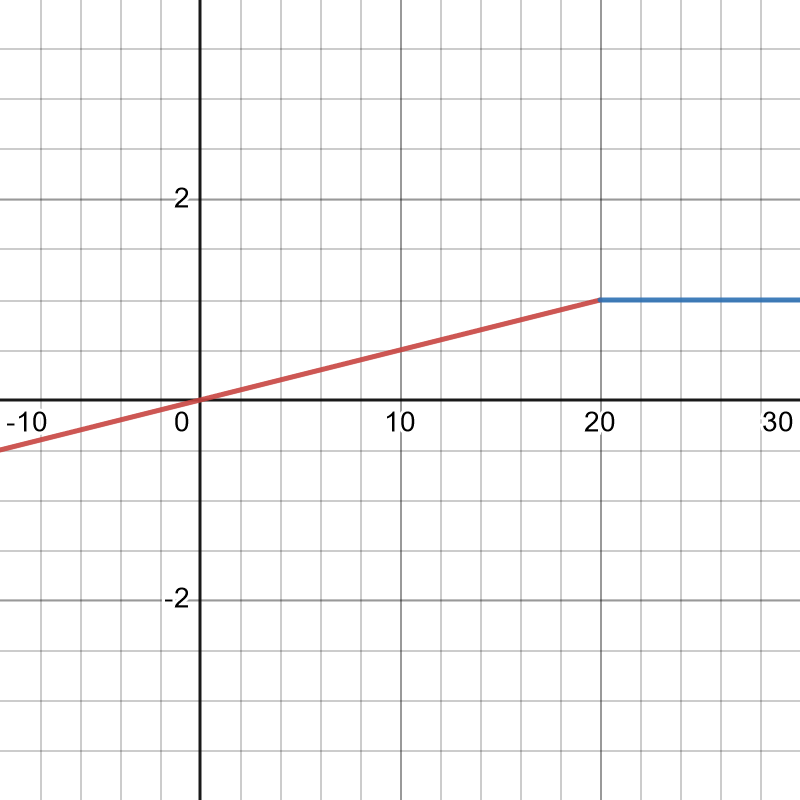
\includegraphics[scale=0.25]{desmos-graph(35).png}
    \end{center}

To the left of twenty, the graph is a line with slope $1/20$; and
to the right of twenty, the graph is a line with slope zero. At twenty,
the graph has a ``corner,'' (no TL), so apparently, the function is not 
differentiable at twenty. Accordingly, we have
\[
    \frac{\mathrm{d}y}{\mathrm{d}x} =
    \begin{cases} 1/20  & x < 20 \\
                 \mbox{dne} & x = 20 \\
                 0 & x >  20 \end{cases}.
\]
    
\end{solution}

\question  In the year 1969 at age 11, child actress Eve Plumb purchased a Malibu beach house for \$55,000. Forty-seven years
later she sold it for \$3.9 million. Her annual percent yield $r$ on this investment is given by the solution to
\[
       3, 900,000 = 55,000 \times (1 + r)^{47}.
\]
Find Eve Plumb's return on this investment. You will need to solve the given equation for $r$.
    \begin{solution}%[3.0in]
        We have
        \begin{align*}
            \left [3, 900,000 = 55,000 \times (1 + r)^{47} \right] &= 
           \left [\frac{780}{11} = (1 + r)^{47} \right] , &\mbox{(divide by 55000)}\\
            &= \left [\left(\frac{780}{11}\right)^{1/47} = (1 + r) \right] , &\mbox{(47th root)}\\
            &= \left [r = \left(\frac{780}{11} \right)^{1/47} - 1 \right], \\
            &= \left [r \approx 9.49\% \right ].
        \end{align*}
    Since 1969, the APY for the S\&P index is about 10.06\%. I'd
    say it was a pretty good investment--of course, the home, unlike
    an S\&P index fund requires upkeep and taxes on homes is different
    than taxes on stock dividends and gains.
    \end{solution}
    \question   After graduation, suppose your starting salary is \$64,000. Further, suppose
that you expect to earn a 3.5\% pay rise each year you work. What is your salary for 
your \nth{40} year of work?  \textbf{Hint:} Your salary for your \nth{3} year of work
is $\$64,000 \times 1.035^2$.
\begin{solution}%[2.5in]
In your \nth{40} year of work, you will have earned 39 pay rises each of 4.1\%. Rounded to 
the nearest penny, your salary for your \nth{40} year of work is
\begin{equation*}
   46,000 \times 1.041^{39} = 220,463.29.
 \end{equation*}   
\end{solution}

\question   Define $Q(x) = x^3 + 1$ and $\dom(Q) = (-\infty,\infty)$. Find the formula
and the domain of $Q^{-1}$. 
\begin{solution} 
    We need to solve $y = x^3+1, -\infty < x < \infty $ for $x$. The
    solution is $x = (y-1)^{1/3}, -\infty < (y-1)^{1/3} < \infty $. 
    Solving $\infty < (y-1)^{1/3} < \infty$ gives $ -\infty < x < \infty$.
    So  $Q^{-1}(y) = (y-1)^{1/3}$ and $\dom(Q^{-1}) = \reals$.
\end{solution}
    \question   Find the \emph{natural domain} of the function $F$ whose
formula is $F(x) = \frac{1}{5+ \frac{1}{x}}$
\begin{solution}%2.5in]
    There are two denominators; we need to require that both are nonzero; thus
    in implicit form, the domain is
    \[
        \dom(F) = \left \{ x | (x \neq 0) \land (5+ \frac{1}{x} \neq 0) \right \}
    \]
    Solving each inequation for $x$ gives and explicit form; it Is
    \[
        \dom(F) = \left \{ x | (x \neq 0) \land (x  \neq -\frac{1}{5}) \right \}.
    \]
    In interval notation, this is
    \[   \dom(F) = (-\infty, -\frac{1}{5}) \cup (-\frac{1}{5},0) \cup
          (0, \infty).
        \]
\end{solution}



\question Find the value of each limit:

\begin{parts}

\part \(\displaystyle \lim_{x \to 0} \frac{x |x|}{x} \).
\begin{solution}
    \[
        \lim_{x \to 0} \frac{x |x|}{x} = 
        \lim_{x \to 0} |x| = 0.
    \]
\end{solution}

\part \(\displaystyle \lim_{x \to 1^{(-)}} \begin{cases} 3 & x < 1 \\ x & 1 \leq x \end{cases}\)
\begin{solution}%[1.5in]
    We're looking at the limit from the \emph{left} toward $1$. That makes
    $x < 1$, so we can simplify \(\begin{cases} 3 & x < 1 \\ x & 1 \leq x \end{cases} \) to $3$.
    Thus
    \begin{align*}
        \lim_{x \to 1^{(-)}} \begin{cases} 3 & x < 1 \\ x & 1 \leq x \end{cases} &=
        \lim_{x \to 1^{(-)}} 3   & \hfill \mbox{(simplification)} \\
        &= 3  &\hfill \mbox{(limit of constant)} \\
    \end{align*}
\end{solution}
\part \(\displaystyle \lim_{x \to 1^{(+)}} \begin{cases} 3 & x < 1 \\ x & 1 \leq x \end{cases}\)
\begin{solution}%[1.5in]
    We're looking at the limit from the \emph{right} toward $1$. That allows us
    to simplify \(\begin{cases} 3 & x < 1 \\ x & 1 \leq x \end{cases} \) to $x$.
    Thus
    \begin{align*}
        \lim_{x \to 1^{(-)}} \begin{cases} 3 & x < 1 \\ x & 1 \leq x \end{cases} &=
        \lim_{x \to 1^{(-)}} x   & \hfill \mbox{(simplification)} \\
        &= 1  &\hfill \mbox{(limit of constant)}) \\
    \end{align*}
    A few of you correctly simplified, but then failed to find the
    limit--something like
    \[
        \lim_{x \to 1^{(-)}} \begin{cases} 3 & x < 1 \\ x & 1 \leq x \end{cases} = x.    
    \]
    OK--there is a pending limit to evaluate. Simplifying is just the
    first step, but we still need to evaluate the limit. 
    
\end{solution}
\part \(\displaystyle \lim_{x \to 1} \begin{cases} 3 & x < 1 \\ x & 1 \leq x \end{cases}\)
\begin{solution}%[1.5in]
    From parts `a' and `b', we have  
    \(\displaystyle \lim_{x \to 1^{(-)}} \begin{cases} 3 & x < 1 \\ x & 1 \leq x \end{cases}
     \neq \lim_{x \to 1^{(+)}} \begin{cases} 3 & x < 1 \\ x & 1 \leq x \end{cases}\), so
     \(\displaystyle \lim_{x \to 1} \begin{cases} 3 & x < 1 \\ x & 1 \leq x \end{cases}\)
     does not exist (aka dne).
\end{solution}

\part \(\displaystyle \lim_{x \to 1} \begin{cases} 3 & x < 10 \\ \ln(x^x + 1)  \sin(1/x) & 10 \leq x \end{cases}\)
\begin{solution}%[1.5in]
    The limit point is $1$. For $x$ near the limit point, we can
    simplify \(\displaystyle \lim_{x \to 1} \begin{cases} 3 & x < 10 \\ \ln(x^x + 1)  \sin(1/x) & 10 \leq x \end{cases}\) to $3$.
    The ugly case  of $10 \leq x$ just ``simplifies away'' and causes us no trouble!
    Thus
    \[
        \lim_{x \to 1} \begin{cases} 3 & x < 10 \\ \ln(x^x + 1)  \sin(1/x) & 10 \leq x \end{cases}
         = \lim_{x \to 1} 3 = 3.
    \]
    
\end{solution}

\part \(\displaystyle \lim_{x \to 5} \frac{\sqrt{x + 2} - \sqrt{7}}{x - 5} \)
\begin{solution}%[1.5in]
    Direct substitution is not an option. To start, let's do some tricky
    algebra:
    \begin{align*}
        \frac{\sqrt{x + 2} - \sqrt{7}}{x - 5} &= \frac{\sqrt{x + 2} - \sqrt{7}}{x - 5} \times \frac{\sqrt{x + 2} + \sqrt{7}}{\sqrt{x + 2} + \sqrt{7}}, \\
           &= \frac{x+2 - 7}{(x-5)(\sqrt{x + 2} + \sqrt{7})}, \\
           &= \frac{1}{\sqrt{x + 2} + \sqrt{7}}.
    \end{align*}
Now the evaluating the limit, is DS:
\[
    \lim_{x \to 5} \frac{\sqrt{x + 2} - \sqrt{7}}{x - 5} 
    =  \lim_{x \to 5}  \frac{1}{\sqrt{x + 2} + \sqrt{7}}
    = \frac{1}{2 \sqrt{7}}
    = \frac{\sqrt{7}}{14}
\]
\end{solution}


\part \(\displaystyle \lim_{x \to \uppi} \frac{\sqrt{x + \uppi} - \sqrt{2 \uppi}}{x - \uppi} \)
\begin{solution}%[1.5in]
This one is not that much different from the previous problem:
\[
    \lim_{x \to \uppi} \frac{\sqrt{x + \uppi} - \sqrt{2 \uppi}}{x - \uppi}
     = \lim_{x \to \uppi} \frac{1}{\sqrt{x + \uppi} + \sqrt{2 \uppi}}
     = \frac{1}{2 \sqrt{2 \uppi}}
\]
\end{solution}

\part \(\displaystyle \lim_{x \to 3} \frac{\sqrt{x + \uppi} - \sqrt{2 \uppi}}{x - \uppi} \)
\begin{solution}%[1.5in]
Ha! This one isn't similar the previous--DS is just fine!
\[
    \lim_{x \to 3} \frac{\sqrt{x + \uppi} - \sqrt{2 \uppi}}{x - \uppi}
    = \frac{\sqrt{3 + \uppi} - \sqrt{2 \uppi}}{3 - \uppi}.
\]
\end{solution}

\part \(\displaystyle \lim_{x \to \sqrt{107}} \frac{x}{|x|}  \)
\begin{solution}%[1.5in]
Near \( \sqrt{107}\), we can simplify \(\frac{x}{|x|}  \) to 1. So
\[
    \lim_{x \to \sqrt{107}} \frac{x}{|x|} = 
    \lim_{x \to \sqrt{107}} 1 = 1.
\]
\end{solution}

\part \(\displaystyle \lim_{x \to -\sqrt{107}} \frac{x}{|x|}  \)
\begin{solution}%[0.0in]
    Near \( -\sqrt{107}\), we can simplify \(\frac{x}{|x|}  \) to -1. So
\[
    \lim_{x \to \sqrt{107}} \frac{x}{|x|} = 
    \lim_{x \to \sqrt{107}} (-1) = -1.
\]
\end{solution}
\end{parts}

\question Find each of the following limits. Use the rules
\begin{description}

    \item[Rule \#0 (constant)] $  \displaystyle \lim_{x \to c} (a) = a$.
     
    \item[Rule \#1 (linearity)] $ \displaystyle \lim_{x \to c} (a F(x) + b G(x)) = a  \, \lim_{x \to c} (F(x)) + b \, \lim_{x \to c} (G(x)) $.
    
    \item [Rule \#2 (product)]$ \displaystyle \lim_{x \to c} (F(x)  G(x)) = \, \lim_{x \to c} (F(x))  \times \lim_{x \to c} (G(x)) $.
    
    \item [Rule \#3 (quotient)] Provided $\displaystyle  \lim_{x \to c} (G(x)) \neq 0$, we have $\displaystyle \lim_{x \to c} \frac{F(x)}{G(x)} = \, \frac{\lim_{x \to c} (F(x))}{ \lim_{x \to c} (G(x)) } $.
    
    \item [Rule \#4 (power)]  $ \displaystyle \lim_{x \to c} F(x)^n  = \left(\lim_{x \to c} F(x) \right)^n  $.
    
    \item [Rule \#5 (root)]  Provided $ \displaystyle  \left(\lim_{x \to c} F(x) \right)^{1/n} $ is real,  $ \displaystyle \lim_{x \to c} F(x)^{1/n}  = \left(\lim_{x \to c} F(x) \right)^{1/n}  $.
    
    \item [Rule \#6 (polynomial)]  Provided $F$ is a polynomial, we have  $ \displaystyle \lim_{x \to c} F(x) = F(c)$
    
     \item [Rule \#7 (rational)]  Provided $F$ is a rational function and $c \in \dom(F)$, we have  \mbox{$ \displaystyle \lim_{x \to c} F(x) = F(c)$.}
    \end{description}

    to justify each of your 
    steps by referencing one of our rules numbered zero through seven.
    
    \begin{parts}
      
        \part  \(\displaystyle \lim_{x \to \uppi} \left(x^3 + x \right) \)
        \begin{solution}%[1.5in]
            Since $x^3 + x$ is a polynomial, we can use Rule 6; thus
            \begin{align*}
                \lim_{x \to \uppi} \left(x^3 + x \right) &= \uppi^3+\uppi. \hfill &\mbox{(Rule 6)}
            \end{align*}
            Alternatively, we could first use Rule 1 (linearity) followed by
            Rule 4; thus
            \begin{align*}
                \lim_{x \to \uppi} \left(x^3 + x \right) &=   \lim_{x \to \uppi} (x^3) +  \lim_{x \to \uppi} (x), \hfill &\mbox{(Rule 1)}\\
                          &= \uppi^3+\uppi. \hfill  &\mbox{(Rule 4, twice)}
            \end{align*}
            To apply Rule 4 to \(\displaystyle \lim_{x \to \uppi} (x)\), match to the 
            algebraically equivalent \(\displaystyle \lim_{x \to \uppi} (x^1)\).
        \end{solution}
          
        \part  \(\displaystyle  \lim_{x \to \sqrt{2}} \sqrt{x+1} \)
        \begin{solution}%[1.5in]
            We have
            \begin{align*}
                \lim_{x \to \sqrt{2}} \sqrt{x+1} &= \sqrt{\lim_{x \to \sqrt{2}} (x+1)}, &\mbox{(Rule 5)} \\
                                                 &= \sqrt{1 + \sqrt{2}}. &\mbox{(Rule 6)}
            \end{align*}
            Since $x+1$ is a polynomial, using Rule 6 in the second step is OK.
        \end{solution}
    
        \part  \(\displaystyle  \lim_{x \to \sqrt{2}} \frac{x+1}{x-1} \)
        \begin{solution}%[1.5in]
            We have
            \begin{align*}
                \lim_{x \to \sqrt{2}} \frac{x+1}{x-1} &= \frac{\sqrt{2}+1}{\sqrt{2}-1},  &\mbox{(Rule 7)} \\
                                                      &= 3 + 2 \sqrt{2}. &\mbox{(simplification)}
            \end{align*}
            The simplification step is done using a multiply by one trick:
            \begin{align*}
                \frac{\sqrt{2}+1}{\sqrt{2}-1} &= \frac{\sqrt{2}+1}{\sqrt{2}-1} \times \frac{\sqrt{2}+1}{\sqrt{2}+1}, 
                \hfill &\mbox{(multiply by one)}\\
                    &= \frac{(\sqrt{2}+1)^2}{2 + \sqrt{2} - \sqrt{2} - 1}, \hfill &\mbox{(distribute denominator)}\\
                    &= \frac{(\sqrt{2}+1)^2}{1}, \hfill &\mbox{(collect like terms)}\\
                    &= 2 + 2\sqrt{2}+1, \hfill &\mbox{(divisor of one)}\\
                    &= 3 + 2 \sqrt{2}. \hfill &\mbox{(collect like terms)}
            \end{align*}
            To earn full credit with our online homework system, generally
            removing radicals from denominator is required.
    
        \end{solution}   
    \end{parts}       
\end{questions}
\end{document}